\section{Fringes as an instrument}
\label{sec:beyond}

Everything so far has treated the index difference $D=\idx_1-\idx_2$ as an
\emph{output}: two families are given, $D$ is whatever they imply, and the fringe
law (Theorem~\ref{thm:fringe}) tells us what we will see. This section runs the
arrow backwards. If the fringes are the unit level sets of $D$, and $D$ is
something we write in a shader, then we may choose the fringes.

\subsection{Encoding a field in the difference}

Let $f:\R^2\to\R$ be any scalar field, and let $a>0$ be a gain. Take a carrier:
any family of phase $\ph_1$ and pitch $s$. Pair it with a second family defined
by
\begin{equation}
  \ph_2(p) \;=\; \ph_1(p) \;-\; a\,s\,f(p).
  \label{eq:encode}
\end{equation}
Both families have the same pitch, so $\idx_i=\ph_i/s$ and
\begin{equation}
  D(p) \;=\; \idx_1(p)-\idx_2(p) \;=\; a\,f(p).
  \label{eq:contourlaw}
\end{equation}
By Theorem~\ref{thm:fringe} the light fringes are $\{D\in\Z\}$, which is
$\{f=n/a\}$: the contours of $f$ at interval $c=1/a$. Not an approximation of
them, and not a discretization of them, but the same curves a contour tracer
would be trying to find. (For a circle-valued $f$ the same construction mints
the quantized defects of \S\ref{sec:defects}.)

Notice everything that does \emph{not} appear. There is no
marching squares, no cell table, no ambiguous saddle, no polyline, no stitching
of segments into curves, no decision about topology, and no resolution at which
any of that would have happened. The contour is never computed. It is a place
where two strokes coincide, and it is drawn by the same distance query and the
same antialiasing the strokes already had.

Because $a$ and $s$ appear only in the product $as$, \eqref{eq:encode} is a
\emph{shift of the phase residual} and nothing else, which is why it costs so
little to ship. \S\ref{sec:catalog} writes every family as $\{\ph=ns+\varphi\}$ and
inks it through $\mathrm{periodicDist}(\ph-\varphi,s)/|\nabla\ph|$; encoding $f$
subtracts $a s f$ inside that residual and subtracts the vector $a s \nabla f$
from the carrier gradient it divides by. Two extra terms, one shared by all
fourteen families (for the concentric and walking families the carrier
direction in that divide is the radial direction from the layer origin, a
first-order convenience).

The gradient term is not optional. Omit it and the modulated family's strokes
thin wherever the field is steep, by the factor $|\nabla\ph_2|$, which is the
same eikonal bug \S\ref{sec:catalog} found in the curve families,
reintroduced through the back door. So a field is not usable unless $\nabla f$
comes with it, which is the whole of the next subsection.

\subsection{Writing the field}
\label{sec:exprs}

$f$ is arbitrary in the mathematics and has to be arbitrary in the tool, or the
contribution reduces to a fixed menu of fields. Our first version was such a
menu: six fields as branches in the shader, each with its gradient
differentiated by hand and transcribed into WGSL and into TypeScript. That is
two derivations and four transcriptions per field, all required to agree and
none checked by a compiler. Adding a seventh field meant editing the renderer, so
neither an author nor we could extend it.

So the tool takes an expression. \texttt{x\^{}2 - y\^{}2} is the saddle,
\texttt{cos(tau * r)} is the bullseye, and $\fieldCount$ presets
(supplemental material, \S S2) are starting points rather than
the offering. The language is deliberately small: the two coordinates, the polar
sugar \texttt{r} and \texttt{theta}, $\pi$, $\tau$ and $e$, the arithmetic
operators with \texttt{\^{}} right-associative, and sixteen functions. There are
no variables, no conditionals and no loops, so a program is a bounded expression
tree and evaluating it is a bounded amount of work, which is what lets it run
per pixel with no schedule and no fallback.

\paragraph{Exact gradients from forward-mode duals.}
Nothing differentiates the expression symbolically. Both evaluators carry a
forward-mode dual number $(v,\partial_x v,\partial_y v)$ through each operation,
so $\nabla f$ falls out of the same traversal that produces $f$, exact to
floating point and never a finite difference. Eq.~\ref{eq:encode} then has the
gradient it needs for the eikonal divide without the author supplying one, and
the hand-derived gradients (the thing most likely to be silently wrong) are
gone. Singular points are handled by clamps shared between the two
evaluators, so a pole is the same finite number on both sides rather than a
\texttt{NaN} on one.

One rule in that traversal deserves stating. In the chain rule $\partial(g\circ h)=g'(h)\,\partial h$, a factor that is
\emph{exactly} zero contributes nothing, even when the other factor
overflowed. A plain multiply gives $0\cdot\infty=\mathrm{NaN}$, and one
\texttt{NaN} anywhere in a gradient poisons the divide in Eq.~\ref{eq:eikonal}
and blanks the layer. The zeros are not rare: a constant's partials are zero, a
coordinate's cross-partial is zero, and $\mathrm{floor}$ and $\mathrm{sign}$
have zero slope everywhere. The CPU evaluator multiplies through a helper that
tests for an exact zero at runtime; the emitter folds the same zeros at compile
time, which covers every structural zero but not a slope that becomes zero only
at runtime behind a domain guard, a divergence we accept and document in the
source. This is the ordinary hazard of automatic differentiation in floating
point, and it is easy to reach here because an author can write
\texttt{log(-1)} into a text box.

\paragraph{Compiling instead of interpreting.}
The bytecode is a stack machine, which invites the obvious implementation: hand
the program to the fragment shader in a uniform buffer and walk it. We did, and it
worked, and it cost $\interpPerOp$\,ms per megapixel \emph{per instruction}:
$\interpHi$ for the longest preset, which at a retina canvas is most of a frame
for one field on one layer of twelve. Worse, an \emph{empty} program cost
$\fieldEmptyCost$, or $\fieldEmptyGain\times$ a kernel with no field machinery at
all, because the shader has to be handed the program before it can discover there
is nothing in it. Every author paid for the feature whether or not they used it.

The fix is to stop interpreting. \texttt{fields/emit.ts} unrolls the bytecode
into straight-line code: the compile-time stack holds the \emph{names} of values
rather than values, so there is no runtime stack, no dispatch, no loop and no
program to pass. \texttt{dup} becomes free: it pushes a name twice. Constants
are spelled into the source where the shader compiler folds them. And the zero
rule above, applied at emission, deletes most of the gradient arithmetic before
it is ever written: a term whose factor is the literal $0$ is not emitted at all,
which is why the $\fieldOpsHi$-instruction programs come out as only
$\fieldStmtHi$ statements. A layer with no field emits nothing.

% GENERATED by paper/tools/numbers.mjs
\begin{table}[t]
  \centering
  \small
  \caption{Cost of one field evaluation per pixel, in milliseconds per megapixel
  on an Apple \texttt{metal-3}. \emph{Interpreted} walks the
  bytecode from a uniform buffer; \emph{unrolled} is that same program compiled to
  straight-line code by \texttt{fields\pslash emit.ts}. Both run in one kernel over
  one set of bindings and are checked against the CPU evaluator at the same points
  before either is timed; they agree with each other to
  $4{\times}10^{-5}$ relative. Each thread evaluates
  the field $32$ times and stores once, so what is timed is the
  arithmetic rather than the store. Interpreted cost is linear in program length;
  compiled cost is not, and \textsc{saddle} compiled is cheaper than the
  $0.0071$ a kernel with no field call at all costs, which is to say it has
  disappeared into the noise.}
  \label{tab:compile}
  \begin{tabular}{@{}lrrrrr@{}}
    \toprule
    Preset & Instr. & Stmts & Interpreted & Unrolled & Ratio \\
    \midrule
    \textsc{saddle} & $7$ & $6$ & $0.771$ & $\mathbf{0.0043}$ & $179\times$ \\
    \textsc{dipole} & $31$ & $40$ & $3.189$ & $\mathbf{0.0213}$ & $150\times$ \\
    \textsc{bumps} & $51$ & $69$ & $5.269$ & $\mathbf{0.0199}$ & $265\times$ \\
    \textsc{swirl} & $67$ & $73$ & $6.865$ & $\mathbf{0.0270}$ & $254\times$ \\
    \textsc{ripple} & $6$ & $11$ & $0.627$ & $\mathbf{0.0156}$ & $40\times$ \\
    \textsc{terrain} & $64$ & $69$ & $6.652$ & $\mathbf{0.0540}$ & $123\times$ \\
    \midrule
    empty program & $0$ & $0$ & $0.044$ & $0$ & --- \\
    no field call & --- & --- & \multicolumn{2}{c}{$0.0071$} & --- \\
    \bottomrule
  \end{tabular}
\end{table}


Table~\ref{tab:compile} prices both generations against each other. Interpreted,
cost tracks program length at $\interpPerOp$ per instruction: the signature of a
dispatch loop, and the reason the feature could not have been open-ended.
Compiled, it stops tracking length and starts tracking content: \textsc{ripple}
is the shortest program in the table and compiles to nearly four times the cost of
\textsc{saddle}, because \texttt{cos(tau * r)} is a hypot and a cosine and almost
nothing else, while \textsc{swirl}'s $\fieldOpsHi$ instructions are mostly
arithmetic the shader compiler can schedule. Over the presets the compiled program is
$\fieldGainLo$--$\fieldGainHi\times$ cheaper, at
$\unrolledLo$--$\unrolledCeil$\,ms per megapixel; the saddle comes in under
$\fieldBaseline$, which is what the same kernel costs with no field call in it at
all. That last entry is not a paradox, it is the resolution of the instrument, and
it is the useful statement: at $\fieldOpsLo$--$\fieldOpsHi$ instructions a field is
no longer a thing the frame budget has to account for.

\paragraph{Two backends, so the emitted code is checkable.}
Unrolling raises an obvious risk: the shader now runs code no human wrote, and
its only reference is an interpreter written in a different language. So the
emitter is backend-agnostic and there are two backends. WGSL ships. A JavaScript
backend exists so the test suite can generate a program, run it, and hold it
against the interpreter on the same inputs without a browser, which is how the
zero rule above was found. On the GPU we check further: the interpreter and the
unrolled code are compiled into the same kernel over the same bindings and
sampled at the same points, and they agree with each other to
$\fieldTwinWorst$ relative and with the \texttt{f64} CPU evaluator to the same
order. Both are verified before either is timed, so a wrong answer cannot be
mistaken for a fast one.

\begin{figure*}[t]
  \centering
  \Description{Three square panels. The first is a dense field of fine black lines
  that curve away from a bright X-shaped region through the center. The second is
  the same state under the envelope view: smooth gray bands forming a hyperbolic
  pattern with a bright cross through the middle, and no fine lines at all. The
  third is the first panel again with thin pink hyperbolae drawn over it, each pink
  curve running along the center of a bright band, and the pink asymptote pair
  crossing at the center.}
  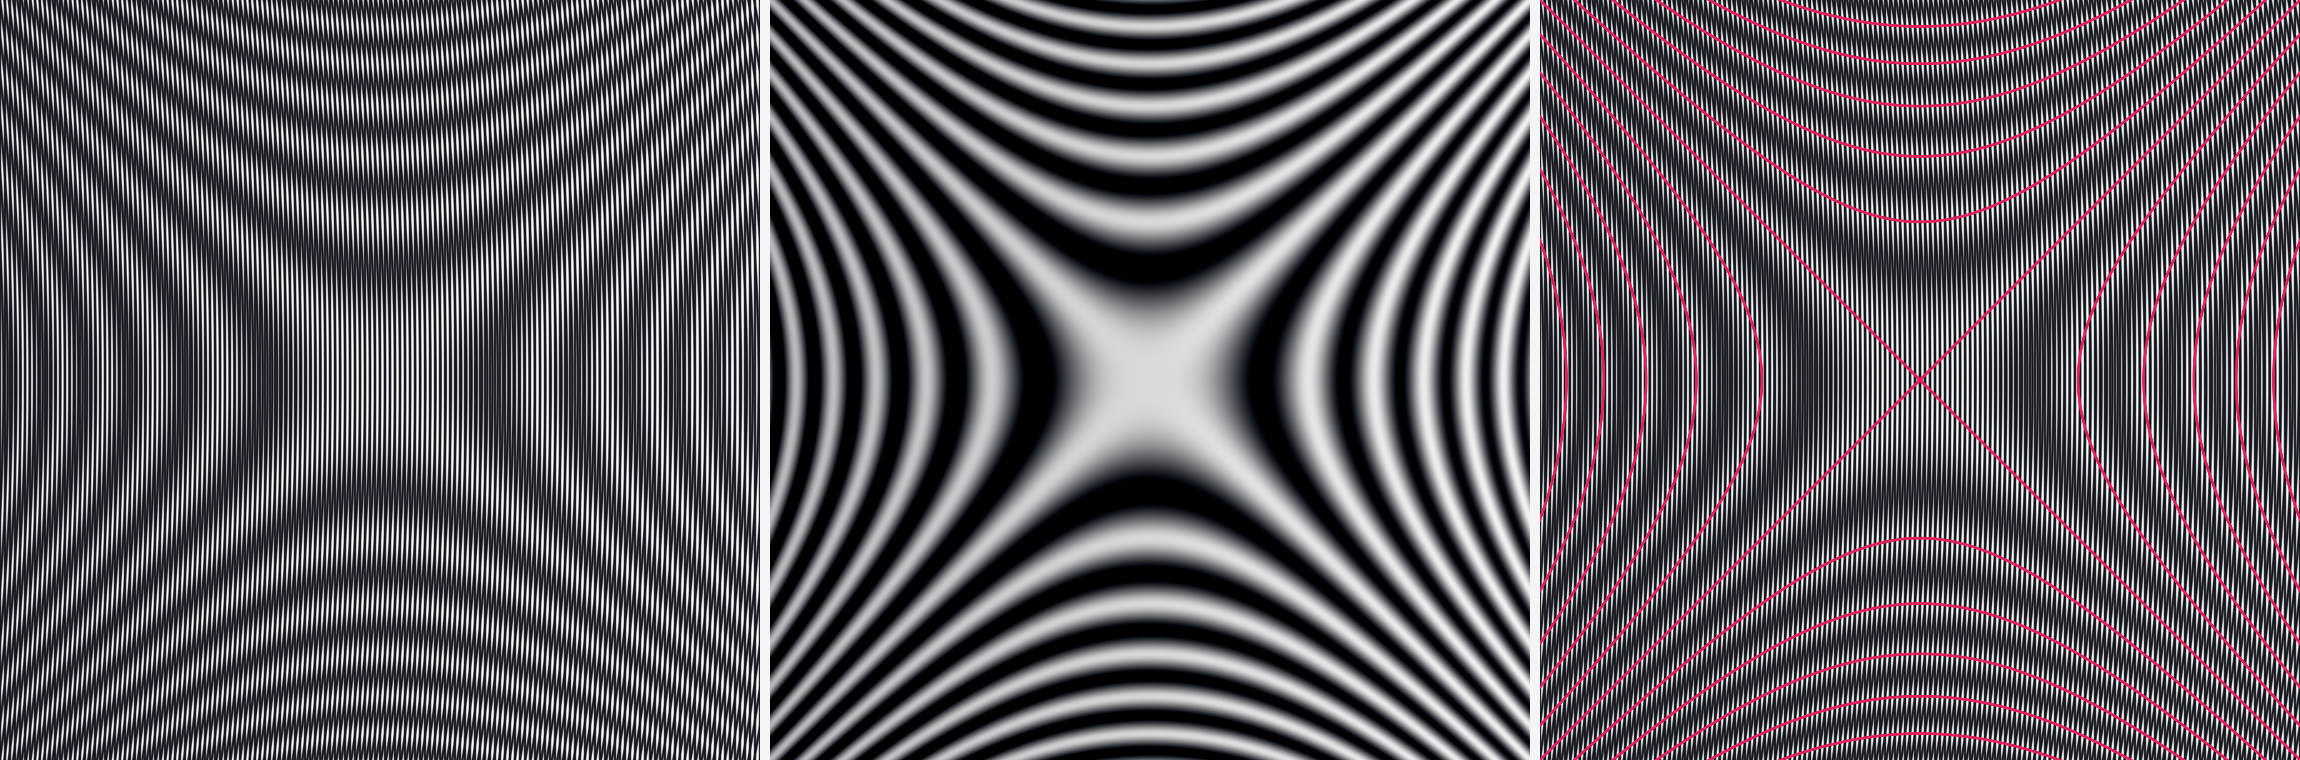
\includegraphics[width=\linewidth]{figures/contour-proof.png}
  \panelrow{0.33043}{0.00435}{%
    (a) as rendered,
    (b) envelope view,
    (c) with the true $\{f=nc\}$}
  \caption{\figlead{A contour plot that was never contoured.} \Moire{}'s
  \textsc{saddle} field encoded by \eqref{eq:encode} into a carrier of pitch
  $\contourCarrier$\,px. \textbf{(a)} The superposition, as rendered: two
  line families and nothing else. \textbf{(b)} The same two layers under the
  envelope view of \S\ref{sec:envelope}: the carrier is gone and the fringe field
  is what is left, its bright bands the level sets of the saddle. This is not a
  blur of (a); it is the mean ink of the same two fields, at the same resolution.
  \textbf{(c)} The rendered image again, with the true curves $\{f=nc\}$ drawn on
  top in pink. They are computed from $f$ alone and laid over a picture that never
  saw them. Note that $f=0$ is the asymptote pair, and the fringe field reproduces
  the crossing.}
  \label{fig:contourproof}
\end{figure*}

\subsection{Does the ink land on the curve?}

Theorem~\ref{thm:fringe} is a statement about a locally averaged quantity, so it
does not by itself promise that the visible bright band of a particular render is
centered on the mathematical curve. That is a question about a rasterized image
and it deserves a measurement rather than an argument.

We measure it as follows. Pick a point, walk it onto the nearest true level set
$\{f=nc\}$ by Newton steps along $\nabla f$ (exact, since \S\ref{sec:exprs}
differentiates every field as it evaluates it) and call the landing
point $q$. Low-pass the render along the carrier direction, enough to erase both
families' strokes and no more, so that nothing is smeared across the fringe we are
about to locate. Then sample that low-passed image along the contour normal
through $q$, fit a parabola to the three samples about the discrete maximum, and
read off the sub-pixel position of the peak. Its displacement from $q$ is the
error, in pixels.

The estimator has a bias of its own, so we calibrate it on a control whose answer
is known in advance, and we pick one that is itself a state of the tool: two
parallel families at pitches $\contourCarrier$ and $\contourDetune$, the oldest
moir\'e there is. Its difference is $x\,(1/s_1-1/s_2)$ exactly, so its fringes are
straight lines $\contourCtlGap$\,px apart. There the measured displacement is
$\contourFloor$\,px on average and $\contourFloorP$\,px at the $95$th percentile,
which is the floor of the method of measurement rather than of the method being
measured.

Against that floor, over $\contourProbes$ probes on the $\fieldCount$ presets of
Figure~\ref{fig:contourfields} (the expressions \Moire{} offers as starting
points, not a set chosen for the experiment), the mean displacement of the
fringe peak from the true contour is
$\contourBestErr$--$\contourWorstErr$\,px, with a worst $95$th percentile of
$\contourWorstP$\,px. That is the strongest statement this
experiment can support: the fringe is on the curve to within our ability to say
where the fringe is.

\begin{figure*}[t]
  \centering
  \Description{Two rows of six square panels. Each panel in the top row is cut
  corner to corner by a black-and-white dashed rule: above the cut is a fine
  black-on-white line texture, below it the same state with the texture gone and
  only broad smooth bands remaining. The six are a hyperbolic cross, two tight
  spiral nests side by side, three merging blobs, four ring nests in a square,
  concentric circles, and an irregular mottled texture. The bottom row shows the
  same six fields as smooth blue-to-yellow heat maps: a saddle, a dipole with one
  dark and one bright pole, three bumps, four vortices, a bullseye, and
  low-frequency noise. Each top panel's bands follow the contours of the map below
  it.}
  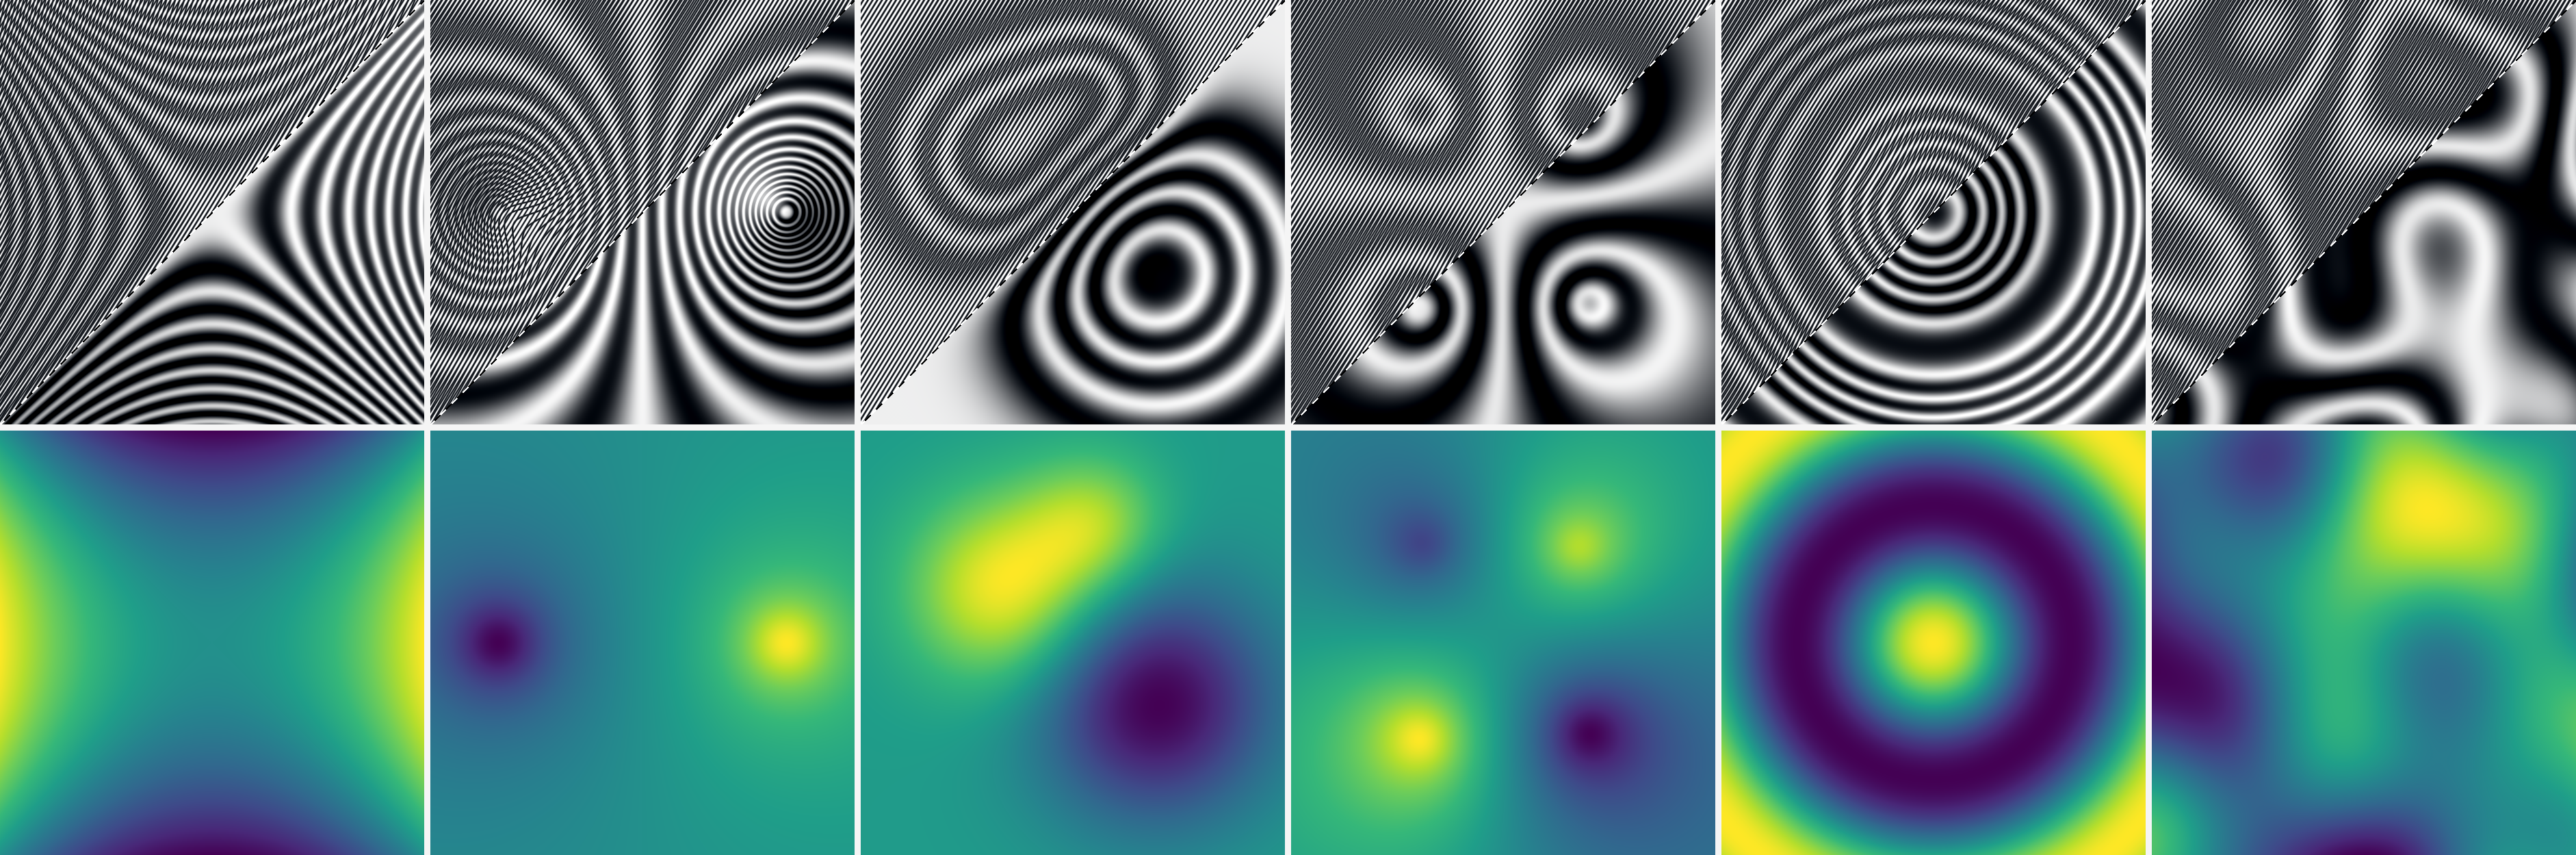
\includegraphics[width=\linewidth]{figures/contour-fields.png}
  \panelrow{0.16467}{0.00239}{%
    saddle, dipole, bumps, swirl, ripple, terrain}
  \caption{\figlead{Every preset the tool ships, encoded.} \emph{Top:} each panel
  is cut corner to corner: the superposition as rendered above the seam, the same
  two layers under the envelope view of \S\ref{sec:envelope} below it. The halves
  are two readings of one state, not two pictures: nothing is filtered between
  them, and the smooth side is the mean ink of the same two fields at the same
  resolution. \emph{Bottom:} the field each one encodes.
  Every pattern above is two \textsc{parallel} layers of pitch
  $\contourCarrier$\,px differing only in one layer's field expression; the labels
  are the presets of \S\ref{sec:exprs}, whose sources are in
  the supplemental material (\S S2). The dipole is instructive: towards each pole the
  equipotentials crowd, and past the limit \eqref{eq:contournyquist} no carrier can
  resolve them, so the render collapses into a dense scribble where the
  field is steepest, which reports the failure rather than hiding it. A contour tracer would emit dense
  polylines there without complaint.}
  \label{fig:contourfields}
\end{figure*}

\subsection{The sampling limit}

The interesting failure is visible in the dipole panel of
Figure~\ref{fig:contourfields}. Fringe spacing is $c/|\nabla f|$, so a field with
a steep region has contours that pack together, and a carrier of pitch $s$ cannot
carry a fringe much finer than itself. Empirically the fringe is legible while
\begin{equation}
  \frac{c}{|\nabla f|} \;\gtrsim\; 3s,
  \label{eq:contournyquist}
\end{equation}
and this is the whole of the method's sampling limit: one inequality, in local
quantities, both of which the renderer already has. It is a Nyquist statement
about the \emph{carrier}, not about the display, which is why raising the zoom
does not help but lowering $s$ does.

Two properties of \eqref{eq:contournyquist} are worth noting. First, it is a field, so it
can be drawn, as the heterodyne ratio of \S\ref{sec:visibility} can:
before committing to $c$, an author can be shown which parts of the frame will
resolve. Second, when it is violated the picture degrades \emph{loudly}. The
unresolvable region fills with visible high-frequency structure (the dipole's
poles turn into a black scribble), which is an honest report that the field is
steeper there than the chosen interval can show. A contour tracer, by contrast, returns a dense set of polylines with no
indication that the interval was too fine for the field.

\subsection{Other uses of the difference}

Equation~\eqref{eq:encode} is one line, and $f$ in it is arbitrary. Several things
follow that we have implemented but not studied, and we record them here
because the field formulation makes them cheap enough to be worth recording.

\paragraph{Streamlines.} A divergence-free planar flow has a stream function
$\Psi$ whose level sets are its streamlines. Encoding $\Psi$ by
\eqref{eq:encode} therefore draws the streamlines of the flow, with no
integration of trajectories, no seeding strategy, and no decision about how long
to trace before stopping. \Moire{}'s \textsc{swirl} field is the stream function
of four point vortices; encoding it draws closed streamlines around each vortex
and the separatrices between them, out of two \textsc{parallel} layers.

\paragraph{Two fields at once.} Two carriers, each with its own encoded partner,
give two independent differences, hence two fringe systems whose crossings are
the joint level sets $\{f=nc_f\}\cap\{g=mc_g\}$. We mention this
with a caveat, because it is where we found the ink budget binds: four dense
families in one frame drive the coverage towards saturation, and the two fringe
systems, though present and correct, are hard to see. Separating them by hue
helps and separating them by pitch helps more, but a clean two-field display
wants a compositing rule other than ``more strokes,'' and we do not have one.

\paragraph{Deformation, which is the classical case.} Let the second family be
the first pulled back through a map $T$, so $\ph_2=\ph_1\circ T$. Then
$D=(\ph_1-\ph_1\circ T)/s$, which to first order is $\langle \nabla\ph_1,
p-T(p)\rangle/s$: the component of the displacement along the family's gradient,
in units of the pitch. The fringes are its contours. This is precisely what
shadow moir\'e, moir\'e topography and moir\'e deflectometry measure with physical
gratings~\cite{Post1994High, Post2008Moire, Takasaki1970Moire}, and it falls out of
\eqref{eq:contourlaw} as the special case $f=\ph_1-\ph_1\circ T$. We note it not
as a new result but as a sanity check on the formulation: the oldest quantitative
use of moir\'e is a corollary of the fringe law, and the amplification factor those
instruments are prized for is the $1/s$ in front. Nothing special is needed to get
it: a vertical carrier and the \textsc{bumps} field is a grating photographed
against its own shadow on a bumpy surface.

\paragraph{Error and disagreement.} Nothing requires $f$ to be a physical field.
Encoding the difference between an approximation and a reference makes the
fringes the contours of the error, at an interval the author sets, in a display
whose ink is legible at any zoom. We found this useful while
debugging the renderer in this paper.

None of this is a new measurement principle; interferometry has used fringe
counting for a century. What is new is where it now sits. These are two extra
terms in a shader in a drawing tool, they run at frame rate, they compose with the
\patternCount{} families of \S\ref{sec:catalog} and with each other, and the
picture they make is a picture---something an author can restyle, zoom, and
put on a page---rather than the output of a measurement pipeline.
